%\documentclass[xcolor=dvipsnames]{beamer}
\documentclass[notes, xcolor=dvipsnames]{beamer}

\usetheme{Warsaw}

\usepackage{inputenc}
\usepackage{graphicx}
\usepackage{amsmath}
\usepackage{amsthm}

\newcommand{\po}{\textcolor{BlueViolet}{po}}
\newcommand{\epo}{\textcolor{BlueViolet}{epo}}
\newcommand{\xpo}{\textcolor{BlueViolet}{xpo}}
\newcommand{\rf}{\textcolor{Green}{rf}}
\newcommand{\co}{\textcolor{BurntOrange}{co}}
\newcommand{\coe}{\textcolor{BurntOrange}{coe}}
\newcommand{\mo}{\textcolor{Red}{mo}}
\newcommand{\hb}{\textcolor{NavyBlue}{hb}}
\newcommand{\fr}{\textcolor{RubineRed}{fr}}
\newcommand{\fre}{\textcolor{RubineRed}{fre}}
\newcommand{\xhb}{\textcolor{NavyBlue}{xhb}}
\newcommand{\rfe}{\textcolor{Green}{rfe}}
\newcommand{\rfi}{\textcolor{Green}{rfi}}
\newcommand{\sw}{\textcolor{BurntOrange}{sw}}
\newcommand{\jhb}{\textcolor{NavyBlue}{jhb}}
\newcommand{\jmo}{\textcolor{Red}{jmo}}
\newcommand{\eco}{\textcolor{WildStrawberry}{eco}}
\newcommand{\rmw}{\textcolor{Bittersweet}{rmw}}
\newcommand{\imp}{\textcolor{LimeGreen}{imp}}


%Misc coloring for binary relations

\title{Robustness Between Weak Memory Models}
\subtitle{Soham Chakraborty}

\author{Presentation by \\ Akshay Gopalakrishnan}

\begin{document}
    
    \begin{frame}

        \maketitle

    \end{frame}

    \begin{frame}{Introduction}

        \begin{itemize}
            \item Robustness is a property that a program can have given two memory models.
            \item A program executing under a memory model $K$ is Robust against memory model $M$ if all consistent executions under $K$ are also consistent under $M$.
            \item This property is useful in ensuring safe portability of programs across different platforms.
            \item However, as far as memory models are concerned, Robustness is maintained only against Sequential Consistency (SC).
            \item This paper analyzes robustness against weaker memory models such as x86-TSO, ARMv7 and ARMv8. 
            \item Robustness conditions are established against each of these models.
            \item An analysis tool is also developed to ensure a program is Robust or if not, adding fence instructions to ensure Robustness.   
        \end{itemize}

    \end{frame}

    \begin{frame}{Examples of Robustness}

        As an example, consider robustness of programs running on ARM against x86. 
        \begin{figure}
            \makebox[\textwidth][c]{
                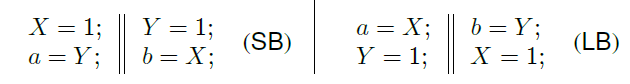
\includegraphics[scale=0.6]{LB_SB_ROBUSTNESS_EX.PNG}
            }
        \end{figure}
        %Explain that TSO exhibits SB but SC does not. Which means SB-TSO is not Robust against SC.
        In the above figure, program SB's outcome $a=1 \wedge b=1$ is allowed by both x86 and ARM. 
        But for the program LB, the outcome $a=1 \wedge b=1$ is allowed by ARM but not by x86.

        Thus, program SB is x86 robust while LB is not. 

    \end{frame}

    \begin{frame}{Robustnes Definition}

        \begin{center}
            \textit{A program P is M-K robust if all its K-consistent executions are also M-consistent.} 
        \end{center}
        
        %Give example of SB program being TSO-ARMv7 robust.
        So for our example above:
        \begin{itemize}
            \item SB is x86-ARM robust.
            \item LB is not x86-ARM robust.
        \end{itemize} 

    \end{frame}

    \begin{frame}{Axiomatic Specification of Memory Consistency Models}

        \begin{itemize}
            \item Define binary relations (mainly partial orders) between program constructs Read/Write/RMW/Fence. 
            \item Per-execution semantics. 
            \item Specify axioms based on relations, which are acyclic/irreflexivity conditions on execution graphs. 
        \end{itemize}

    \end{frame}

    \begin{frame}{Preliminary Definitions of Binary Relations}

        %Put basic ones like po/rf/co/fr
        Binary relations:
        \begin{itemize}
            \item {\po} - Program order per thread.
            \item {\rf} - Between a read and the write from which its read value comes.
            \item {\co} - Order between writes/updates to same location.
            \item {\rmw} - Order between a Read and a Write which form an Atomic update (read-modify-writes).
            \item {\fr} - $\rf^{-1};\co$ read-happens before (also abbreviated as reads-before ).
            \item {\eco} - $\rfe \cup \coe \cup \fre$ called as extended coherence order (take all the external preliminary relations apart from \po).
            \item 
        \end{itemize}


    \end{frame}

    \begin{frame}{SC}

        SC with the above relations can be defined as:
        \begin{itemize}
            \item $\po \ \cup \ \rf \ \cup \fr \ \cup \ \co$ acyclic.
            \item $\rmw \cap \fre;\coe = \phi$.
        \end{itemize}

    \end{frame}

    \begin{frame}{x86-TSO}

        Some additional binary relations (derived)
        \begin{itemize}
            \item {\xpo} - $((W * W) \cup (R * W) \cup (R * R)) \cap \po$ preserved program order.
            \item {\imp} - $\po;[dom(\rmw) \cup F] \cup [codom(\rmw) \cup F];\po$ implied order.
            \item {\xhb} - $\xpo \cup \imp \cup \rfe \cup \fr \cup co$ x86 happens-before.
        \end{itemize}

        x86 is then defined as 
        \begin{itemize}
            \item $\po \ \cup \ \rf \ \cup \fr \ \cup \ \co$ acyclic.
            \item $\rmw \cap \fre;\coe = \phi$.
            \item $\xhb$ acyclic.
        \end{itemize}

    \end{frame}
    

    \begin{frame}{Robustness Conditions: Intuition}

        %mention the Paragraph based intuition on page 4 just before the Robustness conditions.
        The authors tackle only SC, x86-TSO, ARMv7 and ARMv8 models.
        All of the above models respect coherence. 
        If for instance robustness fails to hold, then we have some K-consistent execution to violate an axiom of memory model M.
        Since our axioms are all acyclic/irreflexivity conditions, this implies the execution graph has some form of cycle. 
        Note that, if the cycle contains no {\po} edges, then with the remaining edges ({\rfe}, {\fre}, {\coe}), the cycle also results in coherence violation.
        Thus, the cycle must contain {\po} edges along with the union of the above (now termed as {\eco}).
        This set of {\po} edges are defined as extended program order $\epo = \po \cap (codom(\eco) \times dom{\eco})$. 
        The robustness condition now between each pair of memory model revolves around this newly defined order. 

    \end{frame}

    \begin{frame}{SC-x86TSO Robustness Condition}

        The intuition behind the following theorem is that, we know for certain because of coherence that a cycle if introduced must have {\po} an exclusive part. 
        Thus, it is sufficient to place restrictions on this set of {\po} to belong to a fixed set to ensure no cycle can exist. 
        \begin{theorem}
            A program P is M-K Robust if in all it's K-consistent executions X, $\epo \subseteq R$ where $R$ is defined for each pair of memory models in question.
        \end{theorem}

        For SC-x86TSO robustness $R$ is defined as 
        \begin{align}
            R = \xpo \cup \po_{l} \cup \imp;\po^{?}.
        \end{align}
      
    \end{frame}

    \note{
        


        The intuition behind SC-x86 robustness condition is as follows: 
        \begin{itemize}
            \item {\xpo} orders all R-R, R-W and W-W events. These orders does not actually represent the main weakening that makes it TSO. 
            \item ${\po_{l}}$ If the whole program is surrounding just one memory action, then the program under TSO/SC is the same. 
            \item ${\imp;\po^{?}}$ Any fence between W-R would imply that R will read from the main memory, just like SC semantics. 
        \end{itemize}
        The above three are not the orders that make a Read have a choice to read from its own Write Buffer. 
        This would be different from SC and thus will not be SC-x86 Robust. 
        Thus, we require {\epo} to be in the above union of 3 relations.
    }

    \begin{frame}{Checking and Enforcing Robustness}

        \begin{itemize}
            \item Take the Control Flow Graph of the program.
            \item Build a Memory-access pair graph (MPG) capturing two important edge relations (eco and epo).
            \item If MPG has a cycle, check each access pair whether ordered, as per a condition based on M-K Robustness.
            \item If every pair is ordered, program is M-K Robust.
            \item Else, insert appropriate fences between memory access pairs that are not ordered. 
        \end{itemize}

    \end{frame}

    \begin{frame}{Experimental Evaluation}
        \begin{figure}
            \makebox[\textwidth][c]{
                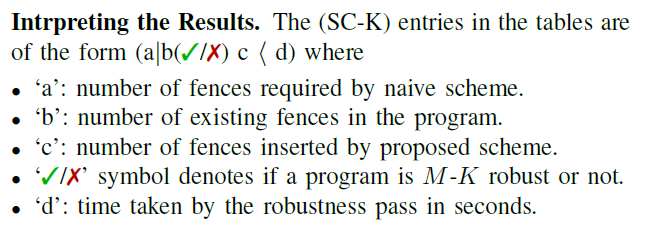
\includegraphics[scale=0.6]{EXP_INTERPRET.PNG}
            }
        \end{figure}
    \end{frame}

    \begin{frame}{Experimental Evaluation Table}
        \begin{figure}
            \makebox[\textwidth][c]{
                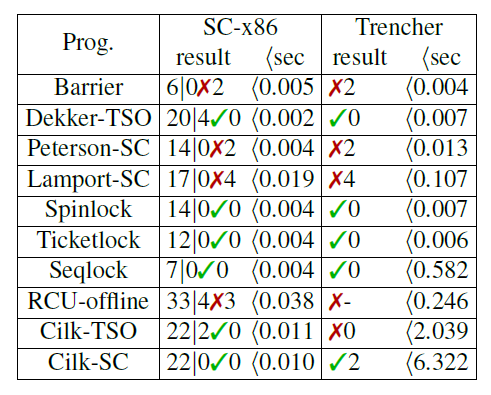
\includegraphics[scale=0.6]{EXPERIMENT_SC-x86.PNG}
            }
        \end{figure}
        Author makes note of Cilk-TSO specifically. 
        Trencher reports violation due to not including ${\po_{l}}$ in condition check. 
    \end{frame}

    \begin{frame}{Thank you}
        Questions?
    \end{frame}


\end{document}